\section{Linear Maps}
\begin{center}
    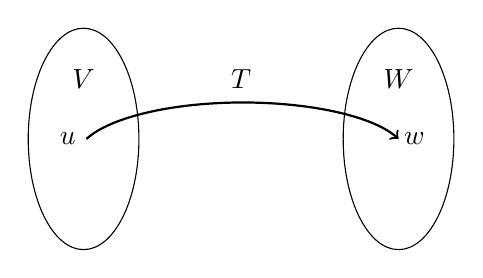
\begin{tikzpicture}
        \draw (2,0) ellipse (20pt and 40pt);
        \draw[] (-2,0) ellipse (20pt and 40pt);
        \draw[<-, thick] (2,0) arc (20:160: 60pt and 20pt);
        \draw (0,1)  node[anchor = north] {$T$};
        \draw (2,1)  node[anchor = north] {$W$}; 
        \draw (-2,1) node[anchor = north] {$V$};
        \draw (-2.2,0) node {$u$};
        \draw (2.2,0) node {$w$};
    \end{tikzpicture}
\end{center}
\subsection{Linear Maps as Vector Space}
Suppose $V$ and $W$ are two linear spaces over $\b F$. $T$ is a function with domain $V$ and codomain $W$. $T$ is called linear iff 
\begin{enumerate}
    \item $T(u_1 + u_2) = T(u_1) + T(u_2)$
    \item $T(\lambda u) = \lambda \cdot T(u)$
\end{enumerate}
$\forall \bar{v}_1, \bar{v}_2 \in V$ and $\forall \bar{v} \in V, \forall \lambda v \in \b F$.
\begin{example}
    Let $V = \b R^3, W = \b R^4$. Define $T$ as $(x_1, x_2, x_3) \mapsto (x_1,0,0,0)$
\end{example}
\begin{example}
    $T: \c P(x) \to \c P(x)$, where $\displaystyle f(x) \mapsto \int_{10}^x f(x) \ dx$ is a linear map.
\end{example}
\begin{definition}
    $\c L\{V, W\}$ denotes the set of all linear maps from $V$ to $W$. Note that $\c L\{V, W\}$ with $+$ and $\cdot$ becomes a vector space over $\b F$. This requires the additions of functions and multiplications of linear maps by scalars (from $\b F$). Given $T_1, T_2 \in \c L(V,W)$ we define addition as $(T_1 + T_2)(u) := T_1(u) + T_2(u)$, multiplication as $(\lambda T)(u) : = \lambda \cdot T(u)$. 
\end{definition}
\begin{theorem}
    In finite vector space $V,W$, let $\li{u}n$ be a basis for $V$, let $\li{w}m$ be any vectors in $W$. Then there exist a unique linear map $T \in \c L \lb V, W \rb$ such that $T(u_j) = w_j \forall j$.
\end{theorem}
\begin{proof}
    Any vector in $V$ has a unique representation $\alpha_1 u_1 + \alpha_2u_2 + \cdots + \alpha_n u_n = u$.  \\ Define $T(u):= \underbrace{\lincomb \alpha {T(u)}n}_{\in W}$ This makes $T$ a linear map from $V$ to $W$. Indeed if $\lambda \in \b F$, then $T(\lambda u) = T(\sum_{j = 1}^n \lambda \alpha_j u_j) = \lambda \sum_{j = 1}^n \alpha_j wj$. Suppose $\tilde T(u_j) = w_j$ for all $j$, then $T = \tilde T$ as a map function by linearity and basis.
\end{proof}
\subsection{Null Space and Range}
\begin{theorem}
    Let $\nul (T):= \lb u \in  v : T(u) = 0 \rb$. $\nul (T)$ is a subspace of $V$.
\end{theorem}
\begin{theorem}
    Let $\range (T):= \lb w \in W : T(u) = w \rb$. $\range(T)$ is a subspace of $W$.
\end{theorem}
\begin{proof}
    The proof is trivial and is left as an exercise for the reader .
\end{proof}
\begin{example}
    Let $T: f \to f', V:= \c P(x), W:= \c P(x)$. $\nul(T) = \c P_0(x)$, $\range(T) = \c P_2(x)$. \\
    Let $T: f \to f'', V:= \c P(x), W:= \c P(x)$. $\nul(T) = \c P_1(x)$, $\range(T) = \c P_1(x)$.
\end{example}
\begin{example}
    Find a basis of $\c L (V,W)$ given bases $\lb \li {u}m \rb$ and $\lb \li{w}n \rb$ of $V$ and $W$. \\
    The basis consists of $m \times n$ vectors as follows: 
    \[T_{11} = T(u_1) = w_1, T(u_2) = 0, T(u_3) = 0, \ldots ,T(u_m) = 0\]
    \[T_{12} = T(u_1) = w_2, T(u_2) = 0, T(u_3) = 0, \ldots ,T(u_m) = 0\]
    \[ \cdots \]
    \[T_{mn} = T(u_1) = 0, T(u_2) = 0, T(u_3) = 0, \ldots ,T(u_m) = w_n\]
\end{example}
\begin{example}
    Let $\c U = \lb f : \b R \to \b R : f(x) = f(1-x) \ \forall x \rb$.
    \begin{enumerate}
        \item Show that $\c U$ is a subspace of $f: \b R \to \b R$. 
        
        \item Find a complement.
        \[ \c W  = \lb g : \b R \to \b R : g(x) = -g(1 - x) \ \forall x \rb\]
        
    \end{enumerate}
\end{example}
\begin{proof}
            We can see that the zero function $f(x) = 0$ satisfies the requirement since $0 = 0$ for all  values of $x$. 
            
            Suppose $f(x), g(x) \in \c U$, then we compute \begin{align*}
                (f + g)(x) &= f(x) + g(x) \\
                           &= f(1 - x) + g(1 - x) \\
                           &= (f + g)(1 - x)
            \end{align*}
            Therefore we can see that $\c U$ is closed under addition.
            
            Suppose $f(x) \in \c U, \lambda \in \b R$, then we compute \begin{align*}
                (\lambda \cdot f)(x) &= \lambda \cdot f(x) \\
                                     &= \lambda \cdot f(1 - x) \\
                                     &= (\lambda \cdot f)(1 - x)
            \end{align*}
            Therefore we can see that $\c U$ is closed addition. 
            Hence $\c U$ is a vector space.
        \end{proof}
\begin{proof}
            The proof for subspace is similar to part (i) and is omitted here. \\
            We now want to show that $\c U + \c W  = \mathbb{R}^{\mathbb{R}}$. We can see that for $f(x) \in \mathbb{R}^{\mathbb{R}}$, we can rewrite $f(x)$ as
            \[ f(x) = \frac{f(x) + f(1 - x)}{2} + \frac{f(x) - f(1 - x)}{2}\]
            Clearly $\displaystyle \frac{f(x) + f(1 -x)}{2} \in \c U$ and $\displaystyle \frac{f(x) - f(1 - x)}{2} \in \c W$. For uniqueness, suppose that a nonzero $h(x) \in \c U \cap \c W$, therefore $h(x) = h(1 - x) = -h(1 - x)$, and the only solution is $f(x) = 0$, a contradiction, therefore $\c U \cap \c W = \lb 0 \rb$. Hence $\boxed{{\b R^{\b{R}}} = \c U \oplus \c W}$
        \end{proof}
\begin{theorem}[Rank-Nullity Theorem also known as the Fundamental Theorem of Linear Maps]
    Let $V,M$ be finite dimensional vector spaces, let $T \in \mathcal L(V,W)$. Then
    \[ \dim V = \dim \nul T + \dim \range T\]
\end{theorem}
\begin{proof}
    Let $\li{u}k$ to be the the basis for the basis for $\nul T$. By the linear independent list extension theory, this list can be extended to a basis of $V$. Say $\li{  u}k, \li{  v}l$ is asujc an extension to a basis of $V$. We can see that $\dim = k + l$. We want to show that $\range T = l$. Consider $\li{T  v}l$. We want to show that $\li{T  v}l$ is basis for $\range T$. Notice that $  v \in V$ can be written as a linear combination of $\lincomb{\alpha}{  u}{k} + \lincomb{\beta}{  v}{l}$. Then we compute \begin{align*}T  v &= \lincomb{\alpha}{T  u}{k} + \lincomb{\beta}{T  v}{l} \\ &= \lincomb{\beta}{T  v}{l} \end{align*} hence $T  u \in \spa (\li{T  v}{l})$. \\
    Suppose $\lincomb{\beta}{T  v}{l} = 0$. Then $\lincomb{\beta}{T  v}{l} \in \nul T$. So \[\lincomb{\beta}{v}{l} = \lincomb{\alpha}{u}{k}\] for some $\li{\alpha}{k}$ since $\li uk$ form a basis for $\nul T$. \\
    But $\li vl, \li vk$ form a basis for $V$, all of the coefficient has to be $0$. Therefore $\li{Tv}k$ is indeed a basis for $\range T$.
\end{proof}
\begin{example}[Direct consequences of the Theorem]
    Suppose $\dim W < \dim V$ (both finite), and $T \in \c L(V,W)$. Then $T$  cannot be injective.
\end{example}
\begin{proof}
    $T$ is injective implies that $\nul T = \lb 0 \rb$. So $\dim V = 0 + \dim \range T \leq \dim W < \dim V$, a contradiction. 
\end{proof}
\begin{example}[Direct consequences of the Theorem]
    Suppose $\dim W > \dim V$ (both finite), and $T \in \c L(V,W)$. Then $T$  cannot be surjective.
\end{example}
\begin{proof}
    $T$ is surjective implies that $\range T = W$. So $\dim V = \dim \nul T + \dim \range T \geq \dim W > \dim V$, a contradiction. 
\end{proof}
\begin{example}[Fun Question]
    Suppose that $p \in \c P(\b R)$, prove that $\exists q \in \c P(\b R)$ such that $5q'' + 3q' = p$. \\
    \noindent [\textit{This exercise can be done without linear algebra, but it’s more fun to do it using linear algebra.}]
\end{example}
\begin{proof}
    Let $d = \deg p$. Define linear transformation $T: \c P_{d +1}(\b R) \to P_d(\b R)$ as $T: q \to 5q''  +3q'$. We can see that $\dim \nul T  = 1$, by the rank nullity theorem, know that $T$ must be surjective as $\dim \c P_{d+1}(\b R) = \dim \nul T + \dim \range T = 1 + \dim \range \implies \dim \range T = \dim P_d(\b R)$.
\end{proof}
\subsection{Matrix Notation}
\begin{center}
    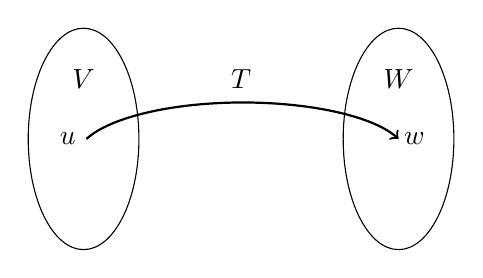
\begin{tikzpicture}
        \draw (2,0) ellipse (20pt and 40pt);
        \draw[] (-2,0) ellipse (20pt and 40pt);
        \draw[<-, thick] (2,0) arc (20:160: 60pt and 20pt);
        \draw (0,1)  node[anchor = north] {$T$};
        \draw (2,1)  node[anchor = north] {$W$}; 
        \draw (-2,1) node[anchor = north] {$V$};
        \draw (-2.2,0) node {$u$};
        \draw (2.2,0) node {$w$};
    \end{tikzpicture}
\end{center}
Recall this diagram, we want to understand $T$ ``correctly". Pick a basis $\li vn$ for $V$ and $\li wm$ for $W$. We can see that $\dim V = n$ and $\dim W = m$. We can define $T$ as
\[Tv_j = A_{1,j} w_1 + A_{2,j} w_2 + \cdots + A_{m,j} w_m \]
Notice that $A$ has the following form
\[ \begin{array}{cc}
     w_1 \to \\
     w_2 \to \\
     \vdots \\
     w_m \to
\end{array}\bml A_{1,1} & A_{1,2} & \cdots & A_{1,n} \\ 
A_{2,1} & A_{2,2} & \cdots & A_{2,n} \\
\vdots & \vdots & \ddots & \vdots \\ 
A_{m,1} & A_{m,2} & \cdots & A_{m,n} \bmr\]
This is called the matrix representation of $T$.
\begin{example}
    Let $D: V \to W$ be defined as $D := p \to p'$. Let $V:= \spa (1, \cos x, \sin x, \cos 2x, \sin 2x) = W$. We can see that 
    \[\begin{array}{rl}
         1 &\hspace{-0.25cm}\mapsto 0 \\ \cos x &\hspace{-0.25cm}\mapsto -\sin x \\ \sin x &\hspace{-0.25cm}\mapsto \cos x \\ \cos 2x &\hspace{-0.25cm}\mapsto -2 \sin 2x \\ \sin 2x &\hspace{-0.25cm}\mapsto \cos 2x
    \end{array} A = \bml 0 & 0 & 0 & 0 & 0 \\ 
               0 & 0 & -1 & 0 & 0 \\
               0 & 1 & 0 & 0 & 0 \\
               0 & 0 & 0 & 0 & -2 \\
               0 & 0 & 0 & 2 & 0 \bmr\]
\end{example}
\subsection{Matrix Representation} 
Recall that if $T$ is a linear transformation
\begin{center}
    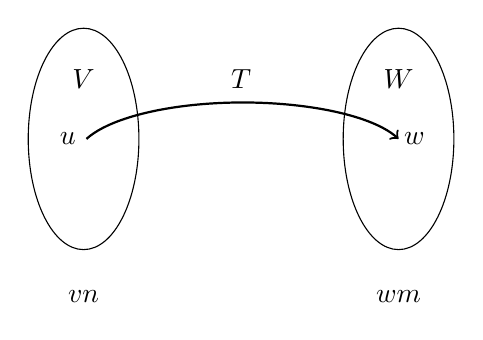
\begin{tikzpicture}
        \draw (2,0) ellipse (20pt and 40pt);
        \draw[] (-2,0) ellipse (20pt and 40pt);
        \draw[<-, thick] (2,0) arc (20:160: 60pt and 20pt);
        \draw (0,1)  node[anchor = north] {$T$};
        \draw (2,1)  node[anchor = north] {$W$}; 
        \draw (-2,1) node[anchor = north] {$V$};
        \draw (-2.2,0) node {$u$};
        \draw (2.2,0) node {$w$};
        \draw (-2, -2) node {$\li vn$};
        \draw (2, -2) node {$\li wm$};
    \end{tikzpicture}
\end{center}
\[ Tv_u = \sum_{k = 1}^{m} A_{i,k} w_k \]
Note that Matrix $A = \left[ A_{i,k} \right]$ has $m$ rows $n$ columns.
\[\left[ \begin{array}{cccc} A_{1,1} & A_{1,2} & \cdots & A_{1,n} \\
        A_{2,1} & A_{2,2} & \cdots & A_{2,n} \\
        \vdots & \vdots & \ddots & \vdots  \\
        A_{m,1} & A_{m,2} & \cdots & A_{m,n} \\
        \end{array} \right]\]
Suppose $v = \lincomb{c}{v}{n}, Tv = \lincomb{c}{Tv}{n}$.
\[Tv =  c_1 \sum_{i=1}^m A_{i,1} w_i  +  c_2 \sum_{i=1}^m A_{i,2} w_i + \cdots + c_n \sum_{i=1}^m A_{i,n} w_n = \sum_{i = 1}^m \left( \sum_{i = 1}^n A_{i,j} c_j \right) w_j \]
Notice that the operation is the equivalent as the matrix-vector multiplication.
\begin{center}
    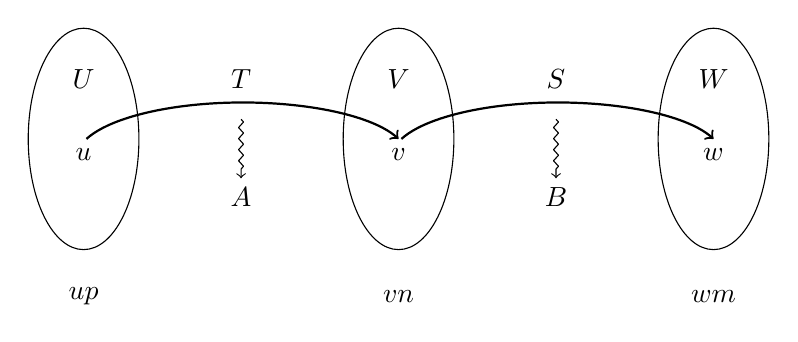
\begin{tikzpicture}
        \draw (2,0) ellipse (20pt and 40pt);
        \draw (-2,0) ellipse (20pt and 40pt);
        \draw (6,0) ellipse (20pt and 40pt);
        \draw[<-, thick] (2,0) arc (20:160: 60pt and 20pt);
        \draw[<-, thick] (6,0) arc (20:160: 60pt and 20pt);
        \draw (0,1)  node[anchor = north] {$T$};
        
        \draw (2,1)  node[anchor = north] {$V$}; 
        \draw (-2,1) node[anchor = north] {$U$};
        \draw (6,1) node[anchor = north] {$W$};
        \draw (4,1) node[anchor = north] {$S$};
        \draw[->, line join=round, decorate, decoration={
    zigzag, segment length=4,
    amplitude=.9,post=lineto,
    post length=2pt }] (0,0.25) -- (0,-0.5);
        \draw[->, line join=round, decorate, decoration={
    zigzag, segment length=4,
    amplitude=.9,post=lineto,
    post length=2pt }] (4,0.25) -- (4,-0.5);
        \draw (0,-0.5) node[anchor = north] {$A$};
        \draw (4,-0.5) node[anchor = north] {$B$};

        \draw (-2,-0.2) node {$u$};
        \draw (2, -0.2) node {$v$};
        \draw (6, -0.2) node {$w$};
        \draw (-2, -2) node {$\li up$};
        \draw (2, -2) node {$\li vn$};
        \draw (6, -2) node {$\li wm$};
    \end{tikzpicture}
\end{center}
\[ STu_k = S(Tu_k) = S \left( \sum_{j=1}^n A_{j,k} v_j \right) = \sum_{j = 1}^{n} A_{j,k} \left(Sv_j\right) = \sum_{j = 1}^n A_{j,k} \sum_{i = 1}^{m} B_{i,j} w_i = \sum_{i = 1}^m \left( \sum_{j = 1}^n B_{i,j}A_{j,k} \right) w_i\]
Use name $\c M(S) := B$, $\c M(T) := A$, $\c M(ST) = BA = \c M(S) \cdot \c M(T)$.
So matrix representation multiply as matrices to produce a composition map or product.
\begin{remark}[Book Keeping]
    $A_{*, j}$ denotes the $j$th column of $A$. \\
    $A_{i, *}$ denotes the $i$th row of $A$.
\end{remark}
Notice that $\c M$ is a linear map, $\c L (V,W) \xrightarrow{\c M} \b F^{m,n}$. 
\begin{proposition}
    $\c M$ is a linear map.
\end{proposition}

\begin{proposition}
    $\b F^{m,n}$ has a basis.
\end{proposition}
\begin{proof}
    Consider $E_{i,j}$, the matrix consists of all zeros with the exception of $1$ in position $(i,j)$. This can be done for all $i = 1, 2, \ldots, m$, $j  =1,2, \ldots, n$. Also notice that $\dim \b F^{m,n} = m \cdot n$
\end{proof}

\subsection{Invertibility and Isomorphism}
\begin{center}
    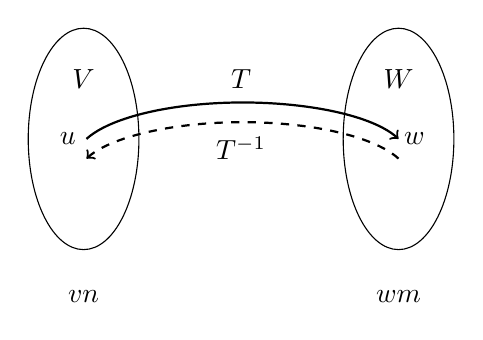
\begin{tikzpicture}
        \draw (2,0) ellipse (20pt and 40pt);
        \draw[] (-2,0) ellipse (20pt and 40pt);
        \draw[<-, thick] (2,0) arc (20:160: 60pt and 20pt);
        \draw[->, thick,style = dashed] (2,-0.25) arc (20:160: 60pt and 20pt);
        \draw (0,1)  node[anchor = north] {$T$};
        \draw (0,0.15)  node[anchor = north] {$T^{-1}$};
        \draw (2,1)  node[anchor = north] {$W$}; 
        \draw (-2,1) node[anchor = north] {$V$};
        \draw (-2.2,0) node {$u$};
        \draw (2.2,0) node {$w$};
        \draw (-2, -2) node {$\li vn$};
        \draw (2, -2) node {$\li wm$};
    \end{tikzpicture}
\end{center}
\begin{definition}
    $T \in \c L(V,W)$ is invertible provided that there exists a mapping $T^{-1}$ from $W$ to $V$ (not necessarily linear) such that \[ T^{-1} \circ T = \b I_V\]
    \[ T \circ T^{-1} = \b I_W\]
    Where $\b I_{V}, \b I_W$ is the identity map on $V$ and $W$.
\end{definition}
\begin{theorem}
    $T$ is invertible if and only if $T$ is both injective and surjective.
\end{theorem}
\begin{proof}
    Suppose $T$ is invertible, then $T(T^{-1} w) = w \ \forall w \in W$, so $\range T = W$. Also we know that $T^{-1}(T v) = v$. Suppose $Tv_1 =Tv_2$, apply the left inverse and we have $T^{-1} (Tv_1) = T^{-1} (Tv_2) \implies v_1 = v_2$. Hence $T$ is injective. Therefore $T$ is bijective. \\
    Now suppose $T$ is bijective. We want to construct $T^{-1}$
    \begin{center}
    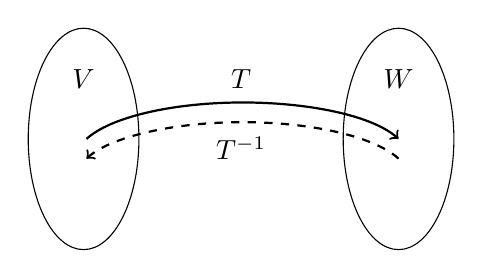
\begin{tikzpicture}
        \draw (2,0) ellipse (20pt and 40pt);
        \draw[] (-2,0) ellipse (20pt and 40pt);
        \draw[<-, thick] (2,0) arc (20:160: 60pt and 20pt);
        \draw[->, thick,style = dashed] (2,-0.25) arc (20:160: 60pt and 20pt);
        \draw (0,1)  node[anchor = north] {$T$};
        \draw (0,0.15)  node[anchor = north] {$T^{-1}$};
        \draw (2,1)  node[anchor = north] {$W$}; 
        \draw (-2,1) node[anchor = north] {$V$};
    \end{tikzpicture}
\end{center}
We need to take $w \in W$, there is a $v \in V$ such that $Tv = w$ and such $v$ is unique since $T$ is injective. We declare $T^{-1}w$ to be $v$. So $T^{-1} \circ T = \b I_{V}$. We compute \[ (T \circ T^{-1}) w = T(T^{-1} w) = Tv = w \ \forall  w \in W\] So $T \circ T^{-1} = \b I_W$ 
\end{proof}
\begin{definition}
    If $V,W$ are vector spaces, such that there exists a invertible linear map $T \in \c L(V,W)$ then $V, W$ are isomorphic.
\end{definition}
\begin{remark}
    Before we proceed, we want to check that $T^{-1}$ is a linear map when $T \in \c L(V,W)$ and $T^{-1}$ exists.
\end{remark}
\begin{proof}
    Take $w_1,w_2 \in W, \lambda \in \b F$. We compute
    $T^{-1} (\lambda w_1 + w_2)$. We know that $w_1 = Tv_1$ and $w_2 = Tv_2$. Then we know that $T(\lambda v_1  + \lambda v_2) = \lambda Tv_1 + Tv_2 = \lambda w_1 + w_2$. Subsitute this into $T^{-1}$ and we get
    \[ T^{-1} (\lambda w_1 + w_2) = T^{-1} \circ T (\lambda v_1 + v_2) = \b I (\lambda v_1 + v_2) = \lambda v_1 + v_2 = \lambda T^{-1} w_1 + T^{-1} w_2\] Hence $T^{-1}$ is linear.
\end{proof}
\begin{corollary}
    $\c M$ is actually a bijection between $\c L(V,W)$ and $\b F^{m,n}$, therefore $\c L(V,W)$ is isomorphic to $\b F^{m,n}$.
\end{corollary}
\begin{theorem}
    Suppose $T \in \c L(V,W)$ is linear and invertible, and let $\li vm$ be a basis for $V$. Then $\li{Tv}n$ is a basis for $W$.
\end{theorem}
\begin{proof}
    Suppose $\lincomb{\alpha}{Tv}{n} = 0$. Then $T(\lincomb{\alpha}{v}{n}) = 0$. Since $T$ is injective, this implies $\lincomb{\alpha}{v}{n} = 0$. Therefore $\alpha_1 = \alpha_2 = \cdots = \alpha_n = 0$ since $\li vn$ is a basis. Take $w \in W$, then there exists a unique $v \in V$ such that $Tv = w$, and $v  =\lincomb{\alpha}{v}{n}$ for some $\li \alpha n$, so $Tv = w = \lincomb{\alpha}{Tv}{n}$, hence span. 
\end{proof}
\begin{corollary}
    $\dim$ is invariant under isomorphism.
\end{corollary}
